% Paper template for TAR 2016
% (C) 2014 Jan Šnajder, Goran Glavaš, Domagoj Alagić, Mladen Karan
% TakeLab, FER

\documentclass[10pt, a4paper]{article}

\usepackage{tar2016}

\usepackage[utf8]{inputenc}
\usepackage[pdftex]{graphicx}
\usepackage{booktabs}
\usepackage{amsmath}
\usepackage{amssymb}


\title{Unsupervised text segmentation}

\name{Mirela Oštrek, Luka Dulčić} 

\address{
University of Zagreb, Faculty of Electrical Engineering and Computing\\
Unska 3, 10000 Zagreb, Croatia\\ 
\texttt{mirela.ostrek@fer.hr}, \texttt{luka.dulcic@fer.hr}\\
}
\abstract{ 
In this paper we describe an unsupervised method for topical segmentation of text. This method represents text as sequence of semantically coherent segments using the Bayesian topic modeling approach and one of the recently developed text segmentation algorithms. We developed and evaluated this method on synthetic Choi dataset. After the initial dataset cleanup, Latent Dirichlet Allocation model is applied to it in order to predict a certain probability distribution over topics which are then used as topic vectors for Topic Tiling algorithm. The latter divides text in semantically coherent segments by calculating cosine similarities and depth scores between the neighboring topic vectors. Performance of this method is evaluated with both $Pk$ and $WD$ measure, and results are shown.
}

\begin{document}

\maketitleabstract

\section{Introduction}
Most people today are searching through digital repositories which contain a great number of documents such as web pages, articles, emails, forum and blog posts, and so on. Despite this information need, finding a relevant topic for a query is extremely difficult task, unless documents are manually annotated with topics \citep{ml-book}. Our aim is to do this annotation automatically and use it to divide a number of documents into semantically coherent units - paragraphs. This will prove to be helpful later on, when search engine tries to retrieve all relevant documents and to pinpoint a specific location in document which best suits user's query.

In order to achieve this claim, we decided to use Bayesian LDA model to predict a probability distribution over topics and Topic Tiling algorithm to segment given text into paragraphs. The former is explained in more detail in Section 3 and the latter is thoroughly described in Section 4. Before the cross validation process, dataset should be properly adjusted and this cleanup step is illustrated in Section 2. In Section 5 we present evaluation results and untangle $Pk$ and $WD$ measures. Section 6 concludes the paper.
More information on this specific method for unsupervised text segmentation can be found in \citep{ref2,ref4,ref-asistent,ref3}. 

\section{Dataset}

\subsection{Choi Dataset description}
The Choi dataset \citep{choi-ref} is commonly used in text segmentation field. It is artificially generated from Brown corpus and consists of 920 documents. Each document consist of 10 segments. Document generation was performed by extracting snippets of 3-15 sentences from different documents from Brown corpus. Documents in Choi dataset are divided into 6 categories based on number of sentences in segments. Categories are 3-5, 3-11, 3-15, 6-8, 9-11, 12-15 where 3-5 indicates there are 3 to 5 sentences in each segment. 
\subsection{Preprocessing}
Preprocessing of Choi dataset consists of standard tasks such as sentence segmentation, tokenization and stemming. Sentence segmentation was easy task because every sentence in Choi dataset is divided by new line character, additionally we needed to remove irrelevant sentences which were empty or consisted of only stop words and other irrelevant tokens. Task of sentence segmentation is essential for this project because Topic Tiling algorithm predicts segment boundaries based on similarities between sentences. Tokenization of sentences was done using standard nltk\footnote{\texttt{http://nltk.org/}} tokenizer. Obtained tokens were then filtered using list of irrelevant tokens which includes standard english stop words list. In further analysis of Choi dataset and experimenting with different lists of irrelevant tokens we decided to also remove all digits, tokens which appeared in more than 95\% of documents or appeared in only one document and some punctuations tokens which were present in dataset but weren't covered with stop words list. This significantly improved performance. After filtering tokens are stemmed using nltk Porter Stemmer. 


\section{LDA}
LDA (Latent Dirichlet Allocation) in text processing is an application of the Bayesian approach, namely topic modeling \citep{ml-book}. It serves its purpose for our method as it outputs probability distribution over topics for each sentence of given text. Topic distribution is assumed to have Dirichlet prior as in:
\begin{equation}\label{eq:dirichlet-prior}
\mathrm{Dirichlet(\theta|\alpha)} = \frac{\Gamma(\alpha_0)}{\prod_i^K \Gamma(\alpha_i)} \prod_i^K \theta_i^{\alpha_i-1},
\end{equation}
where $\theta=[\theta_1, \ldots, \theta_K]^T$ and $\alpha_0 = \sum_i \alpha_i$.
In equation \eqref{eq:dirichlet-prior} $\mathrm{K}$ is the number of topics and $\mathrm{\theta}$ denotes probabilities that correspond to the proportions of different topics. Prior allows us to calculate our prior beliefs in these proportions.

LDA is parametric model and its size is fixed, but we can make this model nonparametric by making the number of topics increase as necessary and adapt to data using a Dirichlet process \citep{ml-book}. However, in our project we did not automatically adjust the number of topics to data. We chose several fixed numbers of topics and evaluated our method against them to see which one gives the most satisfying results. 

LDA model in general works in the following way:
\begin{itemize}
%\setlength{\itemsep}{1pt}
%\setlength{\parsep}{1pt}
%\setlength\parskip{1pt}
\item Generate topics in advance.
\item Assign topic to each word.
\item Check up and update topic assignments iteratively.
\end{itemize}
LDA iterates over the third step defined number of times. This is one of the parameters for fine-tuning LDA model. Other than that, LDA model has three more parameters and those are: $\alpha$ , $\beta$ and number of topics $K$. Parameter $\alpha$ regulates the sparseness of topic-document distribution. Lower values result in documents being represented by fewer topics. Reducing $\beta$ increases the sparsity of topics, by assigning fewer terms to each topic, which is correlated to how related words need to be, to be assigned to a topic \citep{ref-asistent}.

We conducted a research on three different ways of training our LDA model regarding semantically coherent units which are given to LDA as inputs. It is possible to send units such as sentences, paragraphs or even whole documents to LDA, all with goal to fit our model so that it can perform well on set of unseen documents. Inputs for predictions are always sentences because we need to obtain word-topic vectors, which are represented as probability distributions over topics for each sentence, and pass them on to algorithm for text segmentation.


\section{Topic Tiling}
With the aim of being able to segment the given textual document into semantically coherent units, we applied the Topic Tiling algorithm to it. In the previous section we discussed LDA model and how it outputs probability distribution over topics for each sentence of given text. Those outputs are actually called topic vectors and they serve their purpose as inputs for Topic Tiling algorithm. In contrast to some older algorithms for text segmentation such as Text Tiling, Topic Tiling algorithm does not use real words, but it uses topic distribution over words in sentence. 

So, in Topic Tiling algorithm, each sentence of a text is represented by a topic vector. Neighboring topic vectors are then compared in terms of similarity. We decided to use cosine similarity because it is efficient for our task and it is not computationally too expensive. The next step is calculating depth scores $d_p$ with the following expression:
\begin{equation}\label{eq:depth-scores}
\mathrm{d_p} = \frac{1}{2} (hl(p) - c_p + hr(p) - c_p),
\end{equation}
where $hl(p)$ denotes highest peak on the left side of the current depth score point $p$, $hr(p)$ denotes highest peak on the right side of the $p$, and $c_p$ is cosine similarity score calculated for $p$ \citep{ref-asistent}. Figure~\ref{fig:figure1} shows highest left and right peak for certain local minimum.
\begin{figure}
\begin{center}
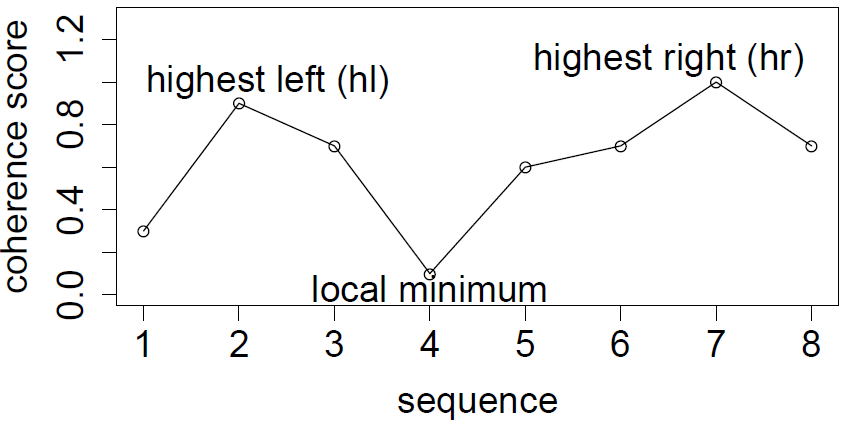
\includegraphics[width=\columnwidth]{depth_scores.jpg}
\caption{Illustration of the highest left and the highest right peak according to a local minimum \citep{ref-asistent}.}
\label{fig:figure1}
\end{center}
\end{figure}
Finally, depth scores are searched for $M$ local minimums, and boundaries are set between topically different segments of text - paragraphs. Number of paragraphs $M$ can be chosen in two different ways:
\begin{enumerate}
%\setlength{\itemsep}{1pt}
%\setlength{\parsep}{1pt}
%\setlength\parskip{1pt}
\item Number is fixed according to developer's "intuition" or already known fact.
\item Number is "calculated" according to certain condition performed on depth scores.
\end{enumerate}

First case is commonly used if we already know how many thematic paragraphs textual document should consist. Second case counts all depth scores which satisfy the following condition as boundaries:
\begin{equation}\label{eq:std-mean}
\mathrm{d_p} > \mu - x \cdot \sigma.
\end{equation}
Condition \eqref{eq:std-mean} must be met for depth score to be marked as boundary between two paragraphs. For that specific purpose, standard mean $\mu$ and standard deviation $\sigma$ are calculated using depth scores as data. In that way, a threshold for depth score being marked as boundary is defined and number of paragraphs is selected dynamically. In condition \eqref{eq:std-mean} there is also $x$ variable present. In our research, we chose a few values for $x$ ranging roughly from $0$ to $1$ to see which is the optimal value of $x$ for dynamical segmentation. Results are shown in the next section.


\section{Performance evaluation}
\subsection{$\mathbf{Pk}$ and $\mathbf{WD}$ measure}
Early articles on text segmentation \citep{hearst-ref} used precision and recall for evaluating segmentation models. These methods are nowadays considered inappropriate for this task because the distance between false positive segment boundary and correct one is not considered at all. For this reason $Pk$ \citep{pk-ref} and $WD$ \citep{wd-ref} measures were developed.

$Pk$ measure uses a sliding window of $k$ tokens which is moved over the text to calculate segmentation penalties. First we generate pairs: $(1, k), (2, k+1), (3, k+2), ..., (n-k, n)$ where $n$ is the length of the document. Then for each pair $(i,j)$ it is checked whether positions $i$ and $j$ belong to same segment. This is done separately for estimated and gold standard boundaries. If the gold standard and estimated boundaries do not match, a penalty of 1 is added. Finally error score is computed by normalizing penalty score by the number of pairs $(n-k)$, which produces number between 0 and 1. A score of 0 indicates perfect match between gold standard and estimated boundaries. The value of parameter $k$ is usually set to half of the average segment length, given by the gold standard.

$WD$ measure is according to its authors Pevzner and Hearst (2002) enhancement over $Pk$ measure, where drawback of $Pk$ is that it is unaware of number of segments between pairs $(i,j)$. First step is the same, dividing document into $(n-k)$ pairs. For each pair $(i,j)$ number of segments between position $i$ and $j$ is counted, separately for gold standard and estimated boundaries. If count for gold standard and estimated boundaries does not match, a penalty of 1 is added, finally error score is obtained by normalizing penalty score by the number of pairs $(n-k)$ which produces number between 0 and 1. A score of 0 indicates perfect match between gold standard and estimated boundaries. 

In practice, $Pk$ and $WD$ measures are highly correlated. For this reason we used only $Pk$ measure for validation of model, to reduce the overhead of parameter grid search, and used both measures for testing model. 

\subsection{Cross validation}
First of all, it is important to note that we were unable to conduct a proper cross validation which is usually mandatory for methods with lot of parameters like this one. Main reason for this is because training of LDA model is very computationally demanding, with certain parameters set, it can take up to 30 minutes. Since we had no high computation hardware available, this was considerable limitation. Because of the latter reasons we were forced to reduce parameters grid search space and to even neglect some parameters for which we used recommended values \citep{ref-asistent}.


Following parameters are subject to optimization in this segmentation model:
\begin{itemize}
\item $K$: Number of topics used in the LDA model. Commonly used values vary from 50 to 500.
\item $\alpha$ : Document topic prior in LDA model. Recommended value is 0.1.
\item $\beta$ : Word topic prior in LDA model. Recommended values are 0.1 or 0.01.
\item $i$ : Inference iterations in LDA model. Recommended value is 70 to 120.
\item $x$ : Multiplier of standard deviation in \eqref{eq:std-mean}. Commonly used value is 0.5.
\end{itemize} 

Parameters $\beta$ and $i$ were not part of grid search. Recommended values $\beta = 0.01$ and $i = 70$ were used. Grid search included parameters $K$, $\alpha$ and $x$ with following values:

\begin{itemize}
\item $K$: $\{60, 80, 100, 120, 130, 140, 150, 160\}$.
\item $\alpha$ : $[0.1, 1]$ with step of 0.1.
\item $x$ : $[0.1, 0.7]$ with step of 0.1. 
\end{itemize}

Beside these parameters, we can also consider LDA input as another parameter. We can input documents, segments or sentences into LDA as mentioned in article before. Again, this parameter was not included in grid search because it would extend grid parameter space considerably. Instead we estimated performance on smaller subset of documents (100) with fixed parameters ($K$=100, $\alpha$=0.1, $\beta$=0.01, $i$=70, $x$=0.5). Input consisting of segments as basic units significantly outperformed other two input types, therefore we used segments as basic input units for model evaluation.

Cross validation was performed with simple train-validation-test split of dataset with ratios of 60:20:20 which indicate percentage of each set. We were unable to use common method of $k$-fold cross validation because of its high computational demand. Table ~\ref{tab:narrow-table} shows segmentation results on validation set.

\begin{table}
\caption{Segmentation results on validation set, for simplicity only scores regarding $x$ parameter is shown with respect of optimal parameters $K$ and $\alpha$.}
\label{tab:narrow-table}
\begin{center}
\begin{tabular}{ll}
\toprule
$K$=150, $\alpha$=0.1 & Pk score \\ 
\midrule
{$x$ = 0.1} & {0.093} \\
{$x$ = 0.2} & \textbf{0.087} \\
{$x$ = 0.3} &{0.095} \\ 
{$x$ = 0.4} & {0.104} \\ 
{$x$ = 0.5} & {0.108} \\ 
{$x$ = 0.6} & {0.122} \\
{$x$ = 0.7} & {0.143} \\ 
\bottomrule
\end{tabular}
\end{center}
\end{table}

\subsection{Results}
Cross validation showed that optimal parameters are: $K$=150, $\alpha$=0.1 and $x$=0.2. $Pk$ measure score for optimal model on test set is 0.09 and $WD$ measure score is 0.1. These results may be suboptimal because of limitations we have faced when conducting model selection. Also these results may vary +-0.02 because of the stochastic nature of LDA model and train-validation-test dataset split. Figure 2 shows segmentation of one randomly chosen document from test set.

\begin{figure}
\begin{center}
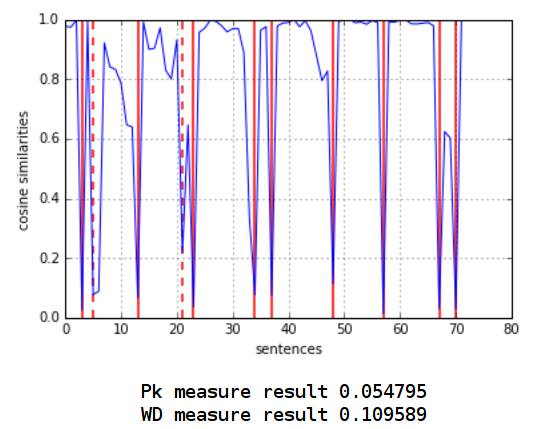
\includegraphics[width=\columnwidth]{plot.png}
\caption{Plot of document segmentation. Blue graph shows cosine similarities between sentences, solid vertical lines indicate correct boundaries and dashed lines indicate false boundaries.}
\label{fig:figure1}
\end{center}
\end{figure}


\section{Conclusion}
Throughout this article we deal with one of the unsupervised methods for text segmentation which is based on the LDA topic model and Topic Tiling algorithm. In the previous section we carefully scrutinized behavior and results which had been conducted upon empowering our method on synthetic Choi dataset. The performance that ensued from cross validation process was fairly satisfying, so we deem this state of the art method to be worthy of its label, but we also imply the need to test it out on sets of real world textual documents. By doing that it would be possible to make proper parameter adjustments and gain new clues on possible correlations between them.


\bibliographystyle{tar2016}
\bibliography{tar2016} 

\end{document}



